%%%%%%%%%%%%%%%%%%%%%%%%%%%%%%%%%%%%%%%%%
% Stylish Article
% LaTeX Template
% Version 2.1 (1/10/15)
%
% This template has been downloaded from:
% http://www.LaTeXTemplates.com
%
% Original author:
% Mathias Legrand (legrand.mathias@gmail.com) 
% With extensive modifications by:
% Vel (vel@latextemplates.com)
%
% License:
% CC BY-NC-SA 3.0 (http://creativecommons.org/licenses/by-nc-sa/3.0/)
%
%%%%%%%%%%%%%%%%%%%%%%%%%%%%%%%%%%%%%%%%%

%----------------------------------------------------------------------------------------
%	PACKAGES AND OTHER DOCUMENT CONFIGURATIONS
%----------------------------------------------------------------------------------------

\documentclass[fleqn,10pt]{SelfArx} % Document font size and equations flushed left

\usepackage[english]{babel} % Specify a different language here - english by default

\usepackage{lipsum} % Required to insert dummy text. To be removed otherwise

\captionsetup[figure]{justification=justified, singlelinecheck=off} 
\captionsetup[table]{justification=justified, singlelinecheck=off} 
%----------------------------------------------------------------------------------------
%	COLUMNS
%----------------------------------------------------------------------------------------

\setlength{\columnsep}{0.55cm} % Distance between the two columns of text
\setlength{\fboxrule}{0.75pt} % Width of the border around the abstract

%----------------------------------------------------------------------------------------
%	COLORS
%----------------------------------------------------------------------------------------

\definecolor{color1}{RGB}{0,0,90} % Color of the article title and sections
\definecolor{color2}{RGB}{0,20,20} % Color of the boxes behind the abstract and headings

%----------------------------------------------------------------------------------------
%	HYPERLINKS
%----------------------------------------------------------------------------------------

\usepackage{hyperref} % Required for hyperlinks
\hypersetup{hidelinks,colorlinks,breaklinks=true,urlcolor=color2,citecolor=color1,linkcolor=color1,bookmarksopen=false,pdftitle={Title},pdfauthor={Author}}

%----------------------------------------------------------------------------------------
%	ARTICLE INFORMATION
%----------------------------------------------------------------------------------------

% \JournalInfo{Journal, Vol. XXI, No. 1, 1-5, 2013} % Journal information
\JournalInfo{$ $ } % Journal information
\Archive{Pre-print} % Additional notes (e.g. copyright, DOI, review/research article)

\PaperTitle{Numerical Instabilities in Analytical Pipelines Compromise the Reliability of Network Neuroscience} % Article title

\Authors{Gregory Kiar\textsuperscript{1}, Yohan Chatelain\textsuperscript{2}, Pablo de Oliveira Castro\textsuperscript{3},
Eric Petit\textsuperscript{4}, Ariel Rokem\textsuperscript{5}, Gaël Varoquaux\textsuperscript{6},
Bratislav Misic\textsuperscript{1}, Tristan Glatard\textsuperscript{2*$\dagger$},
Alan C. Evans\textsuperscript{1$\dagger$}} % Authors
\affiliation{\textsuperscript{1}\textit{Montréal Neurological Institute, McGill University, Montréal, QC, Canada}} % Author affiliation
\affiliation{\textsuperscript{2}\textit{Department of Computer Science and Software Engineering, Concordia University, Montréal, QC, Canada}} % Author affiliation
\affiliation{\textsuperscript{3}\textit{Department of Computer Science, Université of Versailles, Versailles, France}} % Author affiliation
\affiliation{\textsuperscript{4}\textit{Exascale Computing Lab, Intel, Paris, France}} % Author affiliation
\affiliation{\textsuperscript{5}\textit{Department of Psychology and eScience Institute, University of Washington, Seattle, WA, USA}} % Author affiliation
\affiliation{\textsuperscript{6}\textit{Parietal project-team, INRIA Saclay-ile de France, France}} % Author affiliation
\affiliation{*\textbf{Corresponding author}: tristan.glatard@concordia.ca} % Corresponding author
\affiliation{$\dagger$Authors contributed equally}

\Keywords{Stability --- Reproducibility --- Network Neuroscience --- Neuroimaging} % Keywords - if you don't want any simply remove all the text between the curly brackets
\newcommand{\keywordname}{Keywords} % Defines the keywords heading name

%----------------------------------------------------------------------------------------
%	ABSTRACT
%----------------------------------------------------------------------------------------

\Abstract{The analysis of brain-imaging data requires complex and often non-linear transformations to support findings
on brain function or pathologies. And yet, recent work has shown that variability in the choices that one makes when
analyzing data can lead to quantitatively and qualitatively different results, endangering the trust in conclusions.
Even within a given method or analytical technique, numerical instabilities could compromise findings. We instrumented
a structural-connectome estimation pipeline with Monte Carlo Arithmetic and evaluated the stability of the derived
connectomes, their statistics, and the impact on a downstream analysis. The stability of results was found to be highly
dependent upon which features of the connectomes were evaluated, and ranged from perfectly stable (i.e. no observed
variability across executions) to highly unstable (i.e. the results contained no trustworthy significant information).
The extreme range and variability in results presented here could severely hamper our understanding of brain function
in brain-imaging studies. It also highlights both the potential impact of basic analytical choices and measure on the
reliability of downstream analyses, and the necessity of stability evaluation as a core component of typical analytical
workflows.}

%----------------------------------------------------------------------------------------

\begin{document}

\flushbottom % Makes all text pages the same height
\maketitle % Print the title and abstract box
% \tableofcontents % Print the contents section
\thispagestyle{empty} % Removes page numbering from the first page

%----------------------------------------------------------------------------------------
%	ARTICLE CONTENTS
%----------------------------------------------------------------------------------------

\section*{Introduction}

\lipsum[1-3] % Dummy text
 and some mathematics $\cos\pi=-1$ and $\alpha$ in the text\footnote{And some mathematics $\cos\pi=-1$ and $\alpha$ in the text.}.

%------------------------------------------------

\section*{Results}
\lipsum[5] % Dummy text

\begin{figure*}[bth]\centering
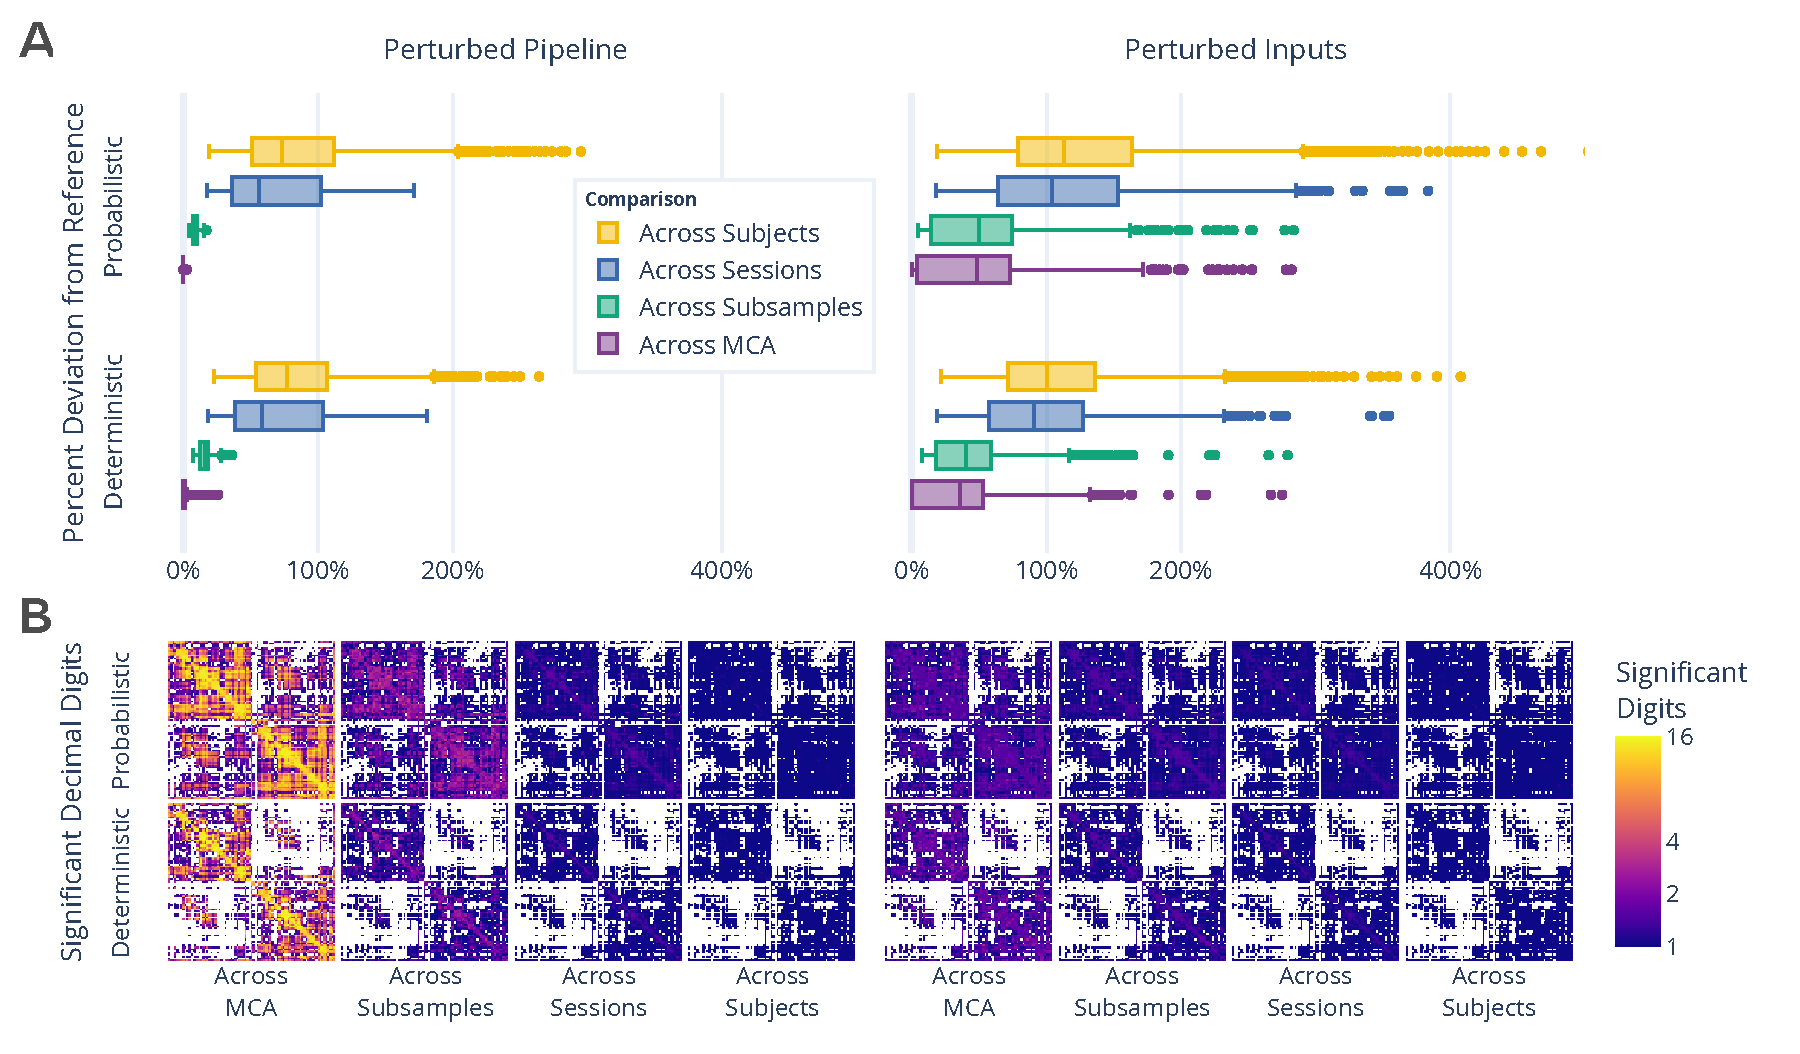
\includegraphics[width=\linewidth]{figures/fig1_absolute_differences.pdf}
\caption{Exploration of perturbation-induced deviations from reference connectomes.
(\textbf{A}) The absolute deviations, in the form of normalized percent deviation from reference, shown as the
across MCA series relative to Across Subsample, Across Session, and Aross Subject variations.
% (\textbf{B}) The correlation between perturbed connectomes and their reference.
(\textbf{B}) The number of significant decimal digits in each set of connectomes as obtained after evaluating the
effect of perturbations. In the case of 16, values can be fully relied upon, whereas in the case of 1 only the first
digit of a value can be trusted. Pipeline- and Input-perturbations are shown on the left and right, respectively.}
\label{fig:absolute}
\end{figure*}

\lipsum[4] % Dummy text

\section{Methods}

\begin{table*}[ht]\centering
\caption{The impact of instabilities evaluated through the separability of the dataset based on simulation, subsample,
session, and subject (reported as mean~$\pm$~standard deviation Discriminability). While a perfectly separable dataset
would be represented by a score of $1.0$, the chance performance is $1 /$the number of classes. In the case of
Hypothesis 1, the evaluation of similarity across individuals, the chance performance is $0.04$. In the case of
Hypotheses 2 and 3, the evaluation of similarity across sessions or subsamples, respectively, the chance performance is
$0.5$. The alternative hypothesis, indicating significant separation across classes, is accepted for all experiments,
with $p < 0.005$.}
\vspace{5pt}
% \fcolorbox{color1}{white}{%
% \parbox{\textwidth-2\fboxsep-2\fboxrule}{\centering
%   \colorbox{color2!10}{
%     \parbox{\textwidth-4\fboxsep-2\fboxrule}{

\begin{tabular}{llll|ll|ll|ll}
  &  &  &  &  \multicolumn{2}{l|}{\textbf{Reference Execution}} & \multicolumn{2}{l|}{\textbf{Perturbed Pipeline}} &  \multicolumn{2}{l}{\textbf{Perturbed Inputs}} \\
Exp. & Subj. & Sess. & Samp. & Det. &  Prob. &  Det. &    Prob. &     Det. &    Prob. \\
% Exp. & Subj. & Sess. & Dirs. & Sims. &     Discrim. (D) &    Discrim. (P) &     Discrim. (D) &    Discrim. (P) \\
\hline
1.1        &          All &      All &          1 &  $ 0.64 \pm 0.00 $ &  $ 0.65 \pm 0.00 $  &  $ 0.82 \pm 0.00 $ &  $ 0.82 \pm 0.00 $ &  $ 0.77 \pm 0.00 $ &  $ 0.75 \pm 0.00 $ \\
1.2        &          All &        1 &        All &  $ 1.00 \pm 0.00 $ &  $ 1.00 \pm 0.00 $ &  $ 1.00 \pm 0.00 $ &  $ 1.00 \pm 0.00 $ &  $ 0.93 \pm 0.02 $ &  $ 0.90 \pm 0.02 $ \\
1.3        &          All &        1 &          1 &        &  &  $ 1.00 \pm 0.00 $ &  $ 1.00 \pm 0.00 $ &  $ 0.94 \pm 0.02 $ &  $ 0.90 \pm 0.02 $ \\
& & & & & & & & & \vspace{-5pt}\\
2.4        &            1 &      All &        All &  $ 1.00 \pm 0.00 $ &  $ 1.00 \pm 0.00 $  &  $ 1.00 \pm 0.00 $ &  $ 1.00 \pm 0.00 $ &  $ 0.88 \pm 0.12 $ &  $ 0.85 \pm 0.12 $ \\
2.5        &            1 &      All &          1 &        &  &  $ 1.00 \pm 0.00 $ &  $ 1.00 \pm 0.00 $ &  $ 0.89 \pm 0.11 $ &  $ 0.84 \pm 0.12 $ \\
& & & & & & & & & \vspace{-5pt}\\
3.6        &            1 &        1 &        All &         &  &  $ 0.99 \pm 0.03 $ &  $ 1.00 \pm 0.00 $ &  $ 0.71 \pm 0.07 $ &  $ 0.61 \pm 0.05 $ \\
\end{tabular}


%     }
%   }
% }%
% }%

\label{tab:discrim}
\end{table*}

\lipsum[4] % Dummy text

\begin{figure*}[tb!]\centering
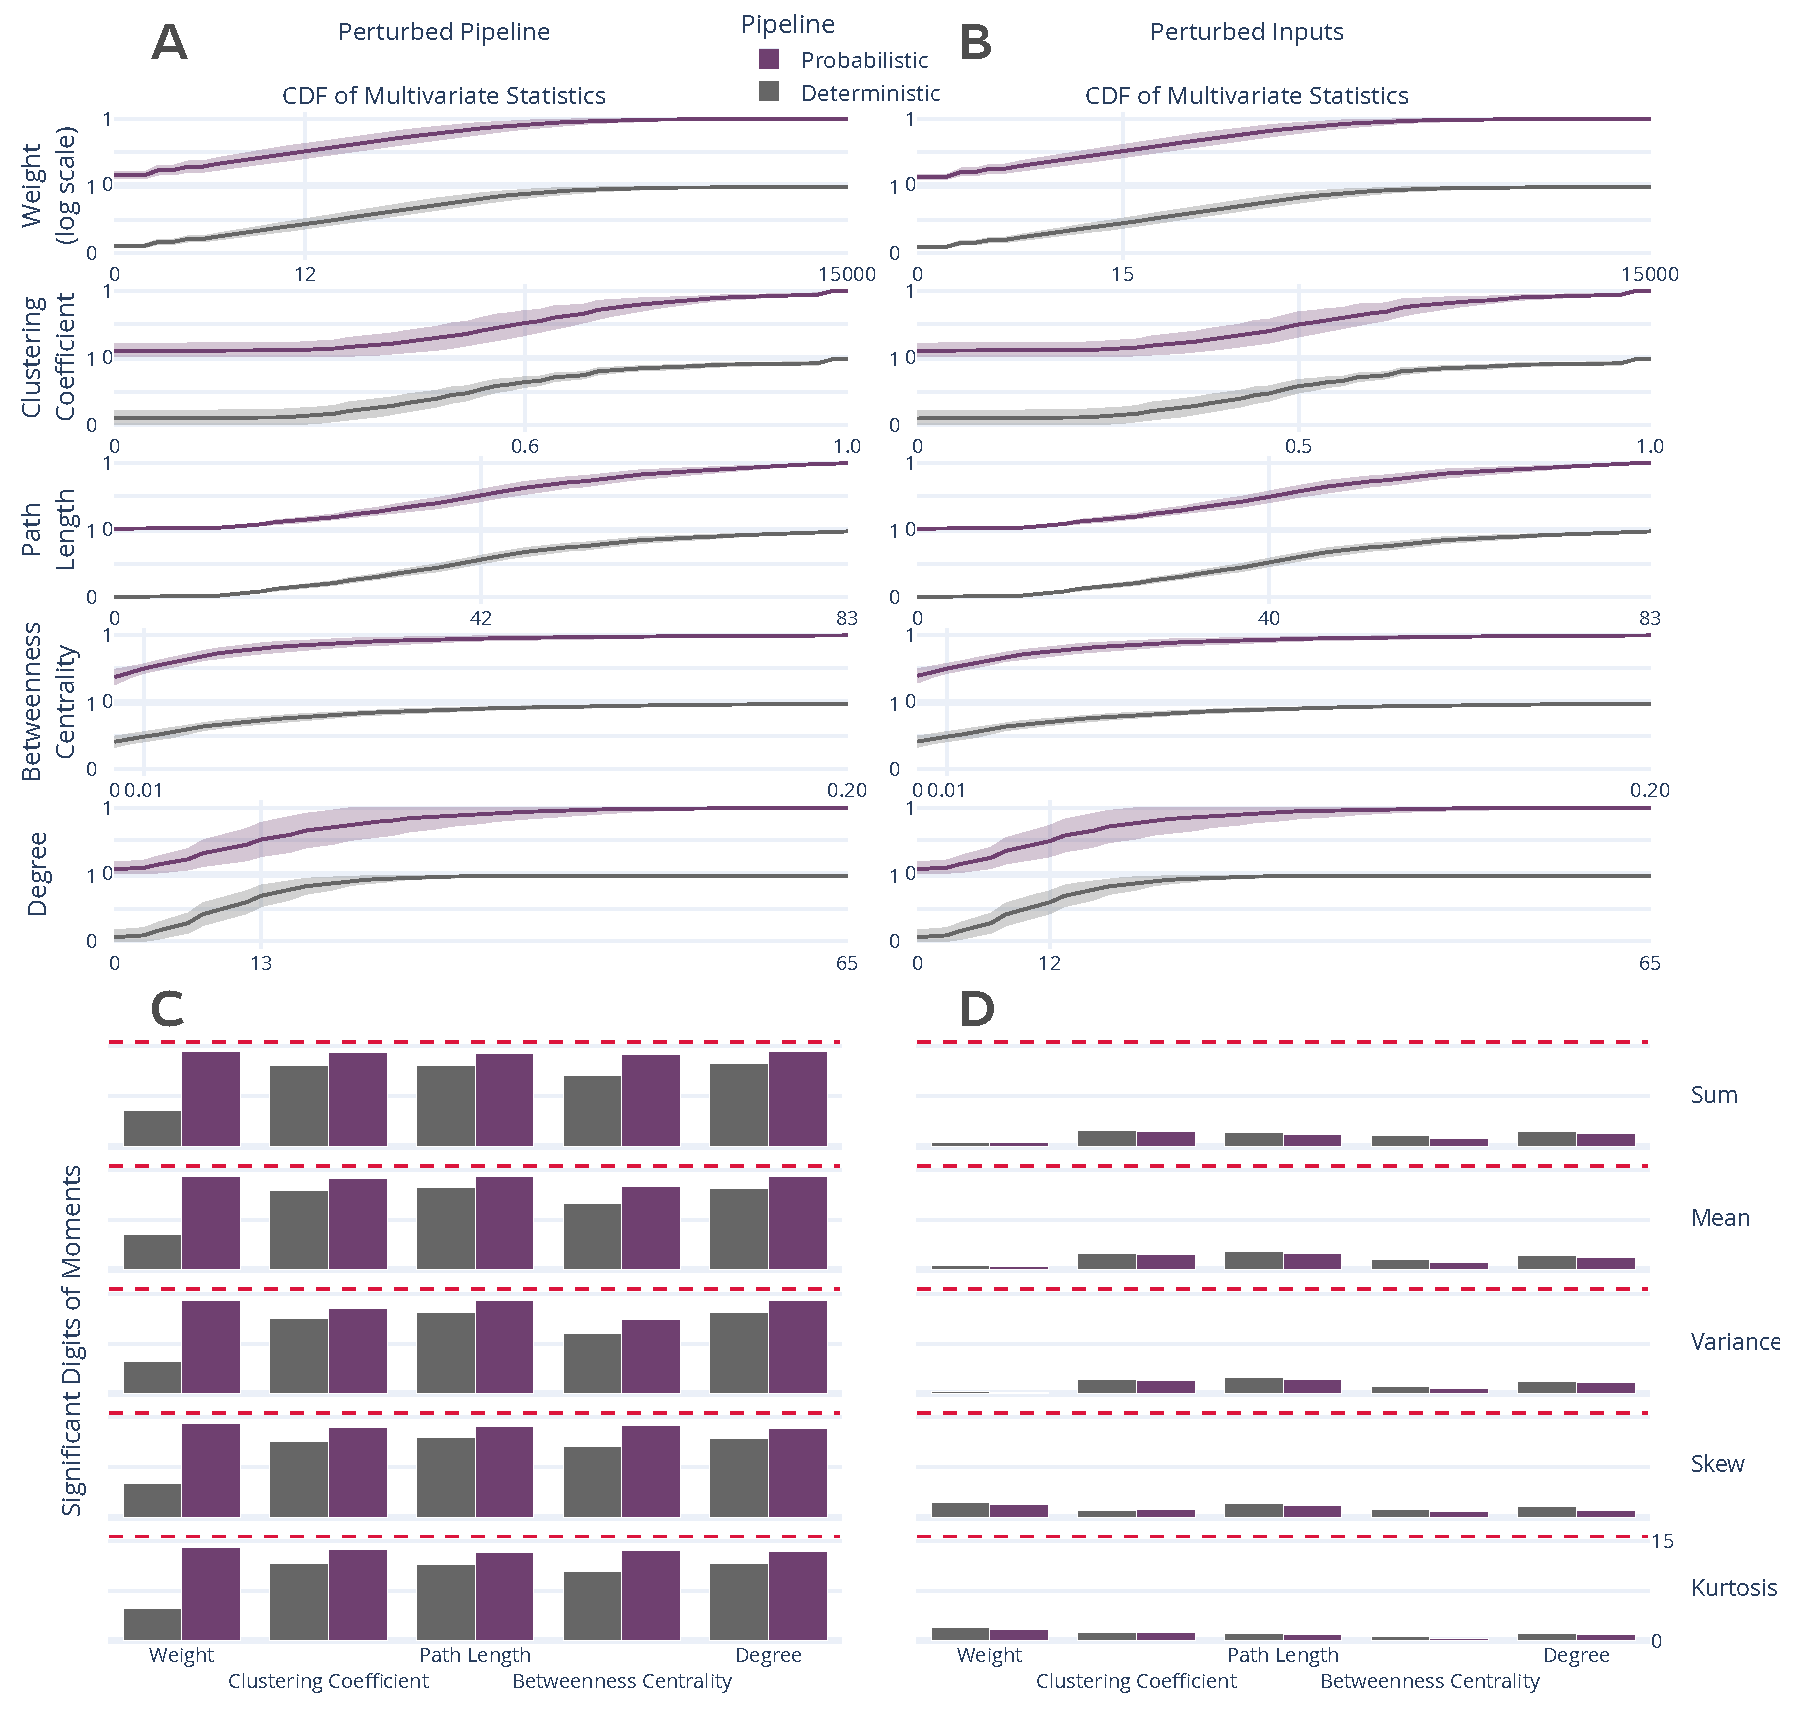
\includegraphics[width=\linewidth]{figures/fig2_multivariate_differences.pdf}
\caption{Distribution and stability assessment of multivariate graph statistics. (\textbf{A}, \textbf{B}) The
cumulative distribution functions of multivariate statistics across all subjects and perturbation settings. There was
no significant difference between the distributions in A and B. (\textbf{C}, \textbf{D}) The number of significant
digits in the first five moments of each statistic across perturbations. The dashed red line refers to the maximum
possible number of significant digits.}
\label{fig:multivar}
\end{figure*}

\lipsum[4] % Dummy text

\begin{figure*}[ht]\centering
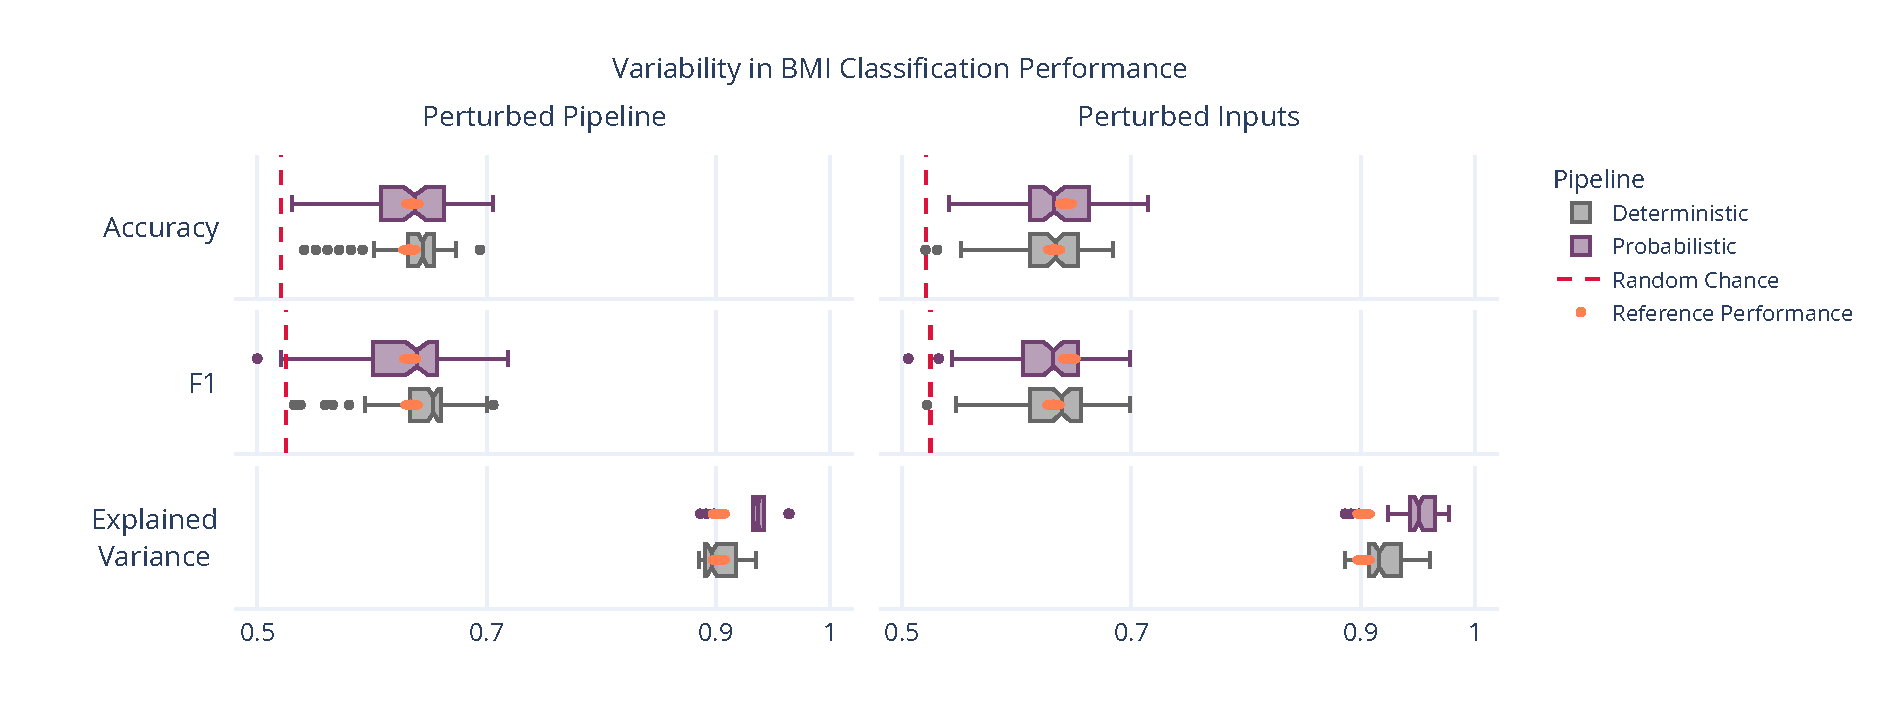
\includegraphics[width=\linewidth]{figures/fig3_bmi_classification.pdf}
\caption{Observed variability in BMI classification. Training and Test sets were sampled from the MCA-generated dataset
such that a single observation of each individual was present in each sampling. This sampling was performed 20 times,
and each dataset was used to train a classifier with each of 2, 5, 10, and N-fold cross validation, and the shown
metrics are the average across each of these training paradigms. The dashed red lines indicate random-chance
performance, and the orange dots show the performance using the reference executions.}
\label{fig:bmi}
\end{figure*}

\begin{equation}
\cos^3 \theta =\frac{1}{4}\cos\theta+\frac{3}{4}\cos 3\theta
\label{eq:refname2}
\end{equation}

\lipsum[5] % Dummy text

\begin{enumerate}[noitemsep] % [noitemsep] removes whitespace between the items for a compact look
\item First item in a list
\item Second item in a list
\item Third item in a list
\end{enumerate}

\subsection{Subsection}

\lipsum[6] % Dummy text

\paragraph{Paragraph} \lipsum[7] % Dummy text
\paragraph{Paragraph} \lipsum[8] % Dummy text

\subsection{Subsection}

\lipsum[9] % Dummy text

Reference to Figure \ref{fig:results}.

%------------------------------------------------

\section{Results and Discussion}

\lipsum[10] % Dummy text

\subsection{Subsection}

\lipsum[11] % Dummy text

\lipsum[15] % Dummy text

\subsubsection{Subsubsection}

\lipsum[12] % Dummy text

\begin{description}
\item[Word] Definition
\item[Concept] Explanation
\item[Idea] Text
\end{description}

\subsubsection{Subsubsection}

\lipsum[13] % Dummy text

\begin{itemize}[noitemsep] % [noitemsep] removes whitespace between the items for a compact look
\item First item in a list
\item Second item in a list
\item Third item in a list
\end{itemize}

\subsubsection{Subsubsection}

\lipsum[14] % Dummy text

\subsection{Subsection}

\lipsum[15-23] % Dummy text

%------------------------------------------------
\phantomsection
\section*{Acknowledgments} % The \section*{} command stops section numbering

\addcontentsline{toc}{section}{Acknowledgments} % Adds this section to the table of contents

So long and thanks for all the fish \cite{Denis2016-wo}.

%----------------------------------------------------------------------------------------
%	REFERENCE LIST
%----------------------------------------------------------------------------------------
\phantomsection
\bibliographystyle{IEEEtran}
\bibliography{impact-of-instability}

%----------------------------------------------------------------------------------------
\beginsupplement

\clearpage
\section{Graph Correlation}
\begin{figure}[ht]\centering
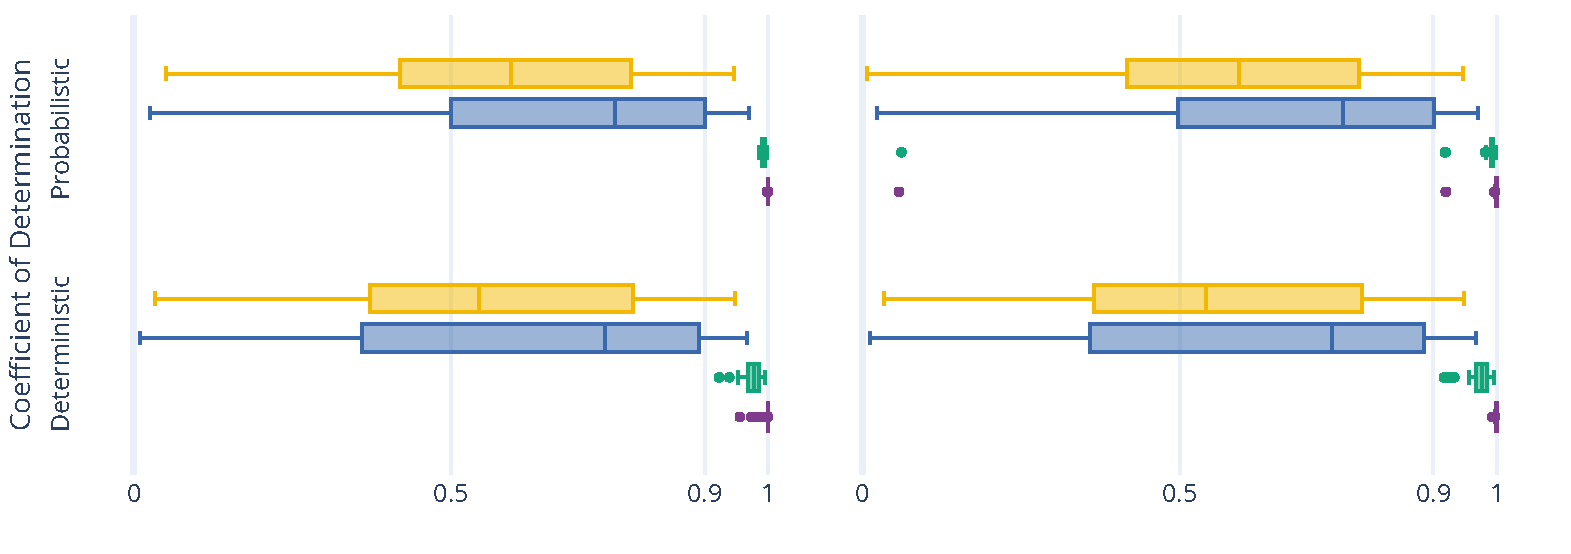
\includegraphics[width=\linewidth]{figures/figS1_correlation_differences.pdf}
\caption{The correlation between perturbed connectomes and their reference.}
\label{fig:bmi}
\end{figure}
words

\clearpage
\section{Univariate Graph Statistics}
\begin{figure}[ht]\centering
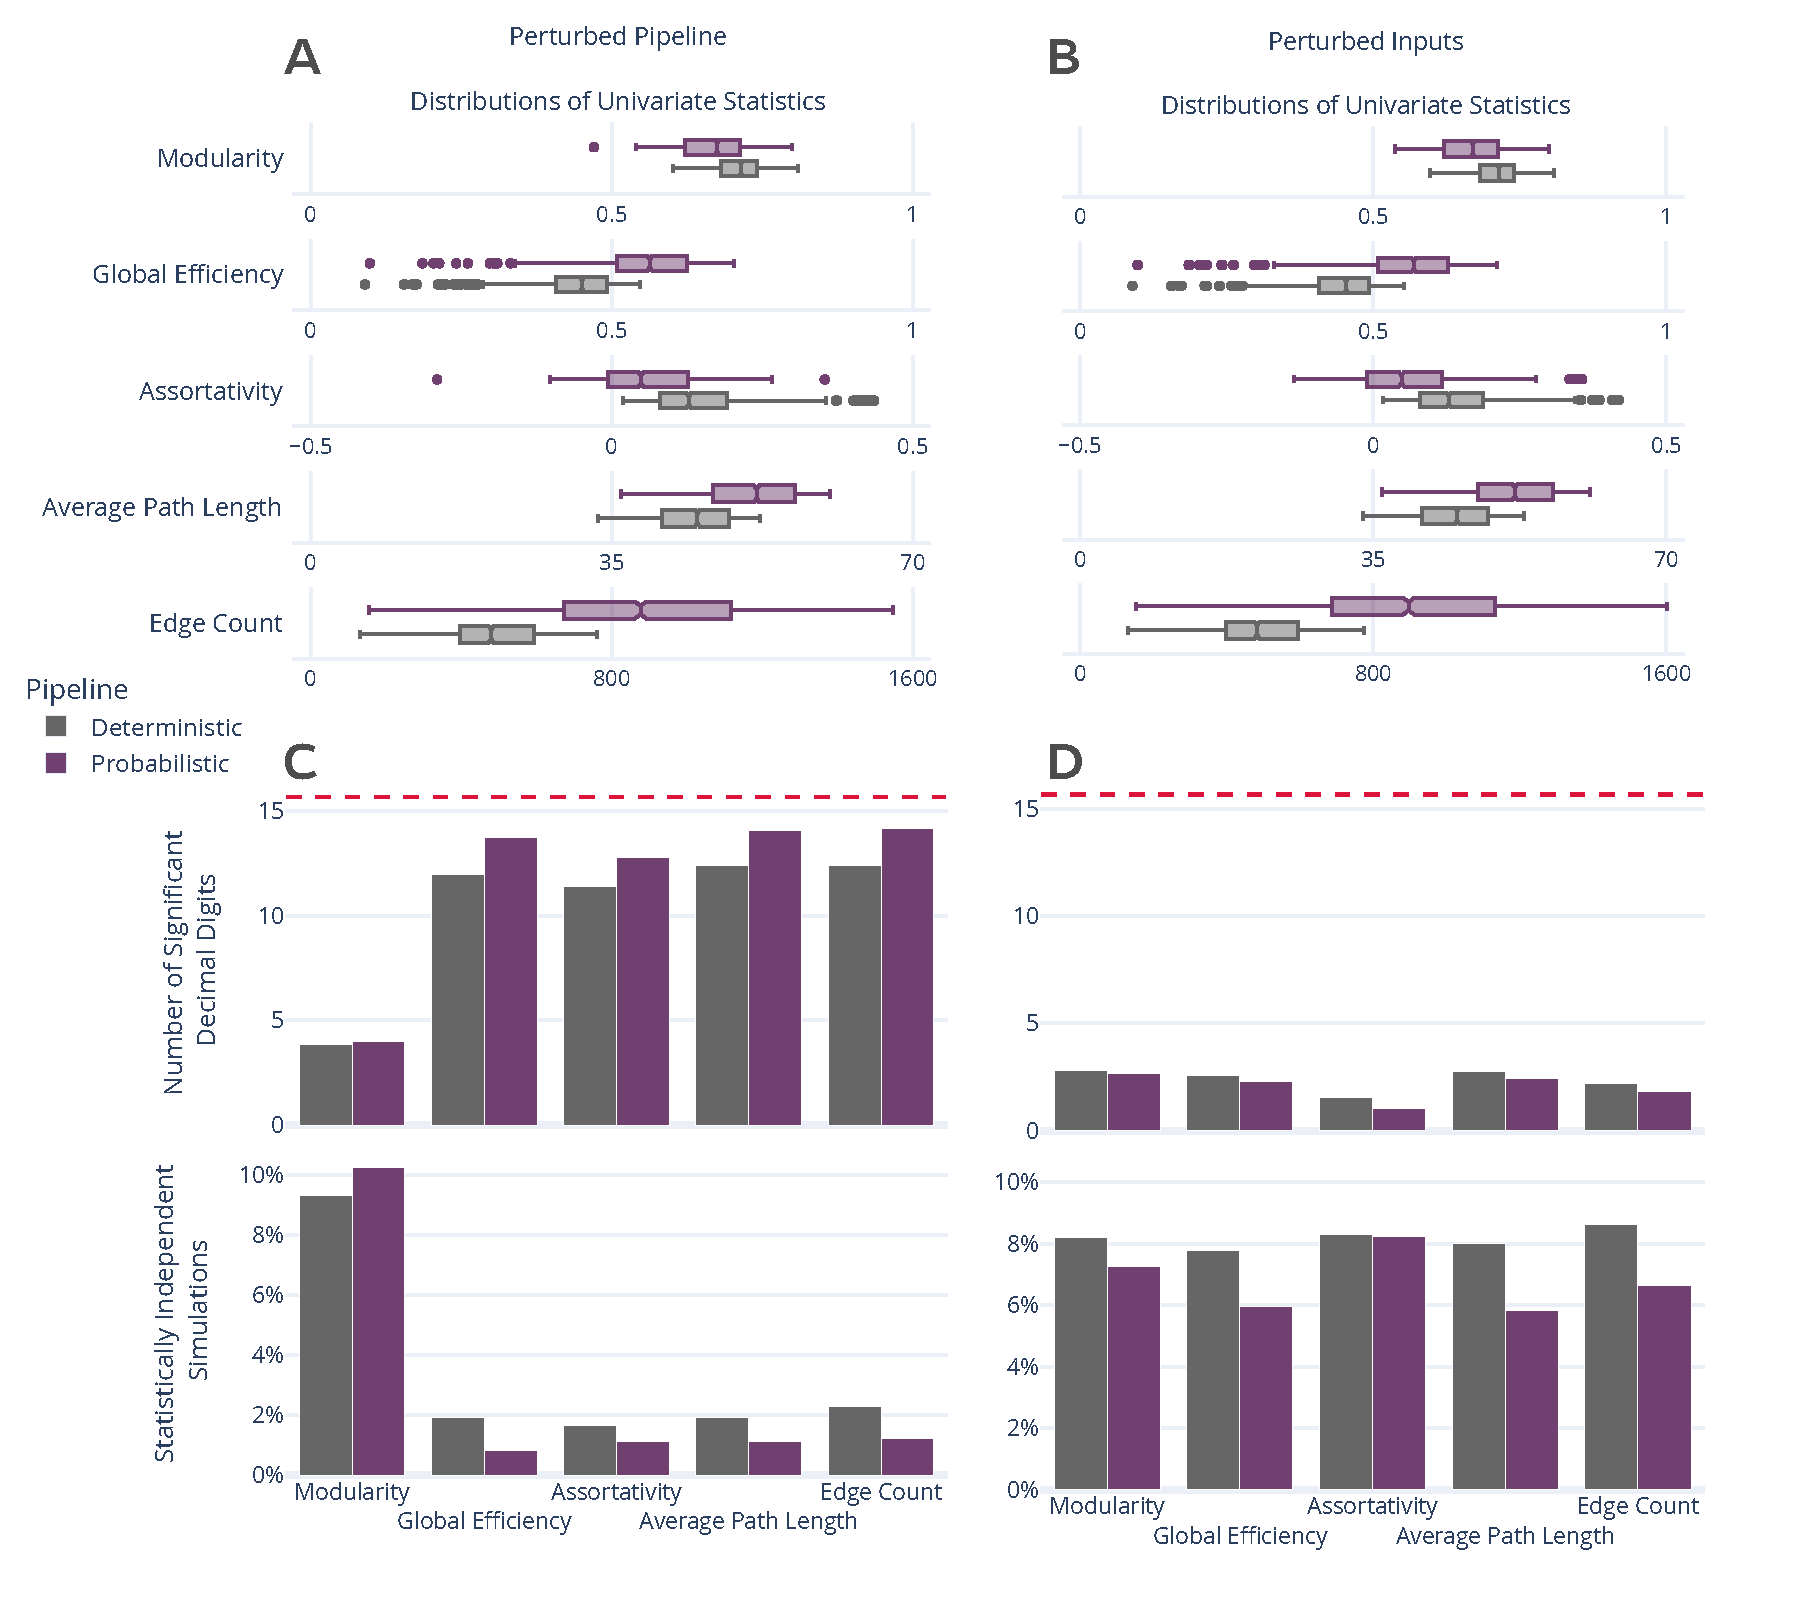
\includegraphics[width=\linewidth]{figures/figS2_univariate_differences.pdf}
\caption{Distribution and stability assessment of univariate graph statistics. (\textbf{A}, \textbf{B}) The
distributions of each computed univariate statistic across all subjects and perturbations for Pipeline and Input
settings, respectively. There was no significant difference between the distributions in A and B. (\textbf{C},
\textbf{D}; top) The number of significant decimal digits in each statistic across perturbations, averaged across
individuals. The dashed red line refers to the maximum possible number of significant digits.
(\textbf{C}, \textbf{D}; bottom) The percentage of connectomes which were deemed significantly different
($p < 0.05$) from the others obtained for an individual.}
\label{sfig:univariate}
\end{figure}
stuff

\end{document}
